%!TEX root = report.tex

\chapter{Cadre Général du Projet}
\section{Introduction}

Ce chapitre est subdivisé en deux parties: la première partie est
consacrée à la présentation de l’organisme d’accueil \textbf{TUNAV}. La
deuxième partie est destinée à la présentation du projet en soit et les
différents facteurs qui ont pesé lors du passage vers la réalisation.

\section{Présentation de l'organisme d'accueil}  

\begin{figure}
\center

\includegraphics[scale=1]{tunav-logo}
\caption{Logo \textsc{Tunav}.}
\end{figure}

TUNAV se situe à la Cité Technologique des Communications, Parc
Technologique El Gazala à l’ARIANA, et a été fondé par son Président
Directeur Général Mohamed Anis Kallel.

En guise de présentation, rien de mieux que de l’avoir directement du patron lui-même\cite{index_tunisie}:

"\textsc{Tunav} est une société technologique, créée au mois d’août
2004, implantée à la technopole El Gazala et spécialisée dans la
technologie GPS et ses diverses applications dans les domaines de
navigation et de gestion de flotte."

"\textsc{Tunav} est connue en Tunisie par son système \og{}LaTrace\fg{}
de gestion de flotte par GPS, lequel a été commercialisée pour la
première fois en Octobre 2005. Il s'agit d'un système articulé autour
d'une application très évoluée de gestion de flotte, d'une gamme
d'appareils GPS/GPRS et d'une base de données géographique richement
renseignée."

\textsc{Tunav} possède un savoir faire reconnu dans le domaine de la
localisation qui peux être exploité dans le domaine médical.

\section{Présentation du projet}

\subsection{Utilisateurs Cibles}

Cette application vise \underline{principalement} les médecins. Et
malgré que, suite à des choix conceptuels, rien n’empêche qu’avec des
modifications minimes une audience plus large dans le corps médical
pourra être ciblée, ce n’est pas -pour le moment- le but de
l’application. Les médecins, malgré leur formation prolongé dans le
domaine médical, représente une cible sans une vrais profondeur
technique, ce que requière de l’application d’être le plus simple
possible.

\subsection{Spécification des Besoins}

\subsubsection{Besoins fonctionnels}

\begin{figure}
\center
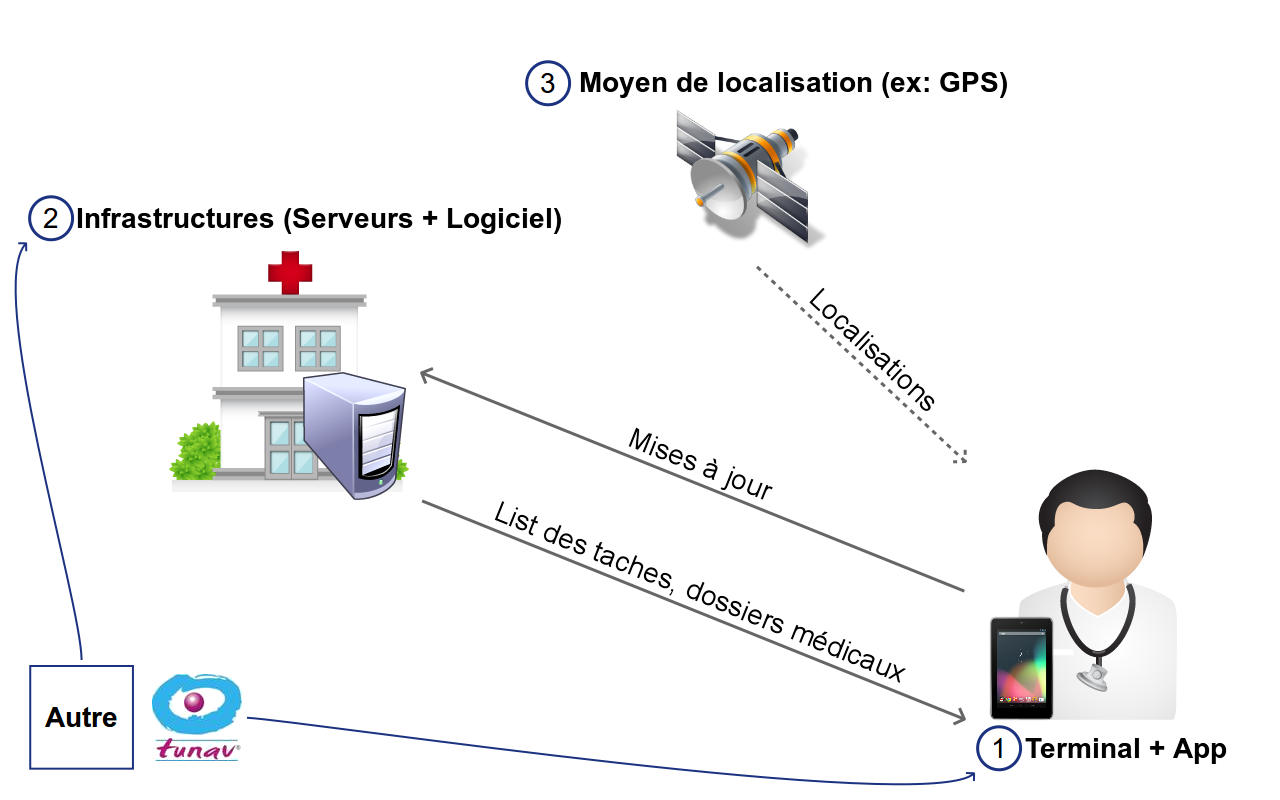
\includegraphics[width=0.8\textwidth]{scenario-other}
\caption{Illustration des besoins fonctionnels.}
\end{figure}

\begin{itemize}

\item Le médecin doit être capable à partir de son terminal d’avoir des
informations sur les patients qui lui sont assigné en fonction de leur position
géographique.

\item L'application doit être capable de détecter la proximité d'un
patient en fonction de la position actuelle du terminal.

\item Le médecin peut télé-consulter le dossier médical du patient.

\end{itemize}

\subsubsection{Besoins non fonctionnels}

\begin{itemize}

\item Une bonne ergonomie qui vise à faciliter l'obtention de
l'information, avec un minimum d'effort pour l'utilisateur cible et
avec le moindre risque d'erreur. Les choix graphiques et conceptuels
sont des considérations à tenir en compte.

\end{itemize}

\subsubsection{Besoins techniques}

\begin{figure}
\center
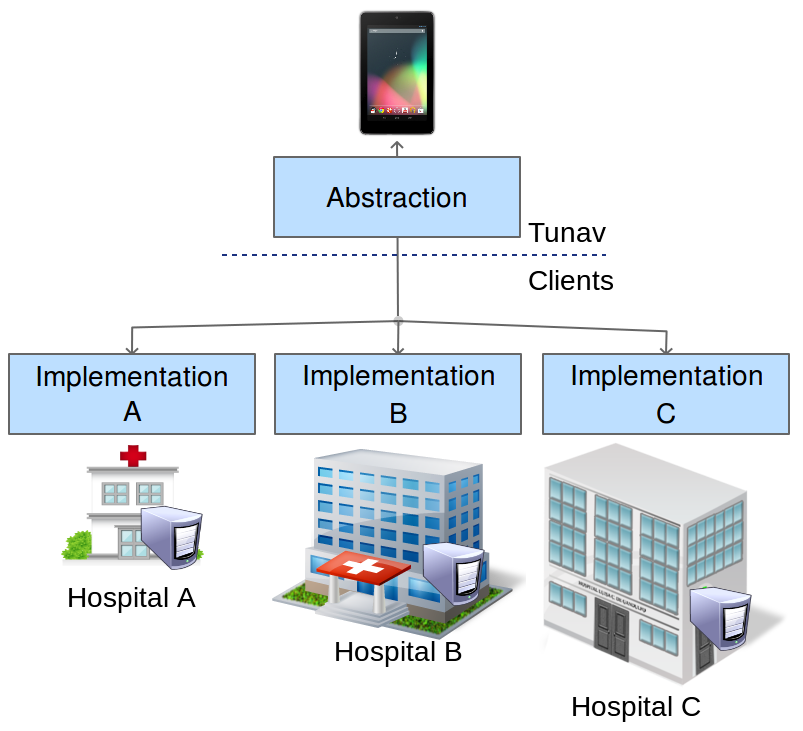
\includegraphics[width=0.8\textwidth]{architecture-interfaces}
\caption{Illustration des besoins techniques.}
\end{figure}

\begin{itemize}

\item L’application mobile vise à utiliser les systèmes déjà en place des
établissements clients pour réduire les coûts. Vu l’absence d'un protocole
standards et les différentes implémentations possibles des différents clients,
l'implémentation d'une couche d’accès abstraite est requise pour pouvoir
déployer l’application avec le minimum de modification.

\end{itemize}

\section{Conclusion} 

La présentation de l'entreprise nous à permis de mieux cerné les points
forts qu'on pourrait compter sur pendant le développement de notre
solution. Et une connaissance exhaustive des objectifs de ce projet
offre une base solide nécessaire pour éviter de s’engager dans des
fausses pistes.
